\documentclass[12pt,]{article}
\usepackage{lmodern}
\usepackage{amssymb,amsmath}
\usepackage{ifxetex,ifluatex}
\usepackage{fixltx2e} % provides \textsubscript
\ifnum 0\ifxetex 1\fi\ifluatex 1\fi=0 % if pdftex
  \usepackage[T1]{fontenc}
  \usepackage[utf8]{inputenc}
\else % if luatex or xelatex
  \ifxetex
    \usepackage{mathspec}
  \else
    \usepackage{fontspec}
  \fi
  \defaultfontfeatures{Ligatures=TeX,Scale=MatchLowercase}
\fi
% use upquote if available, for straight quotes in verbatim environments
\IfFileExists{upquote.sty}{\usepackage{upquote}}{}
% use microtype if available
\IfFileExists{microtype.sty}{%
\usepackage{microtype}
\UseMicrotypeSet[protrusion]{basicmath} % disable protrusion for tt fonts
}{}
\usepackage[margin=1in]{geometry}
\usepackage{hyperref}
\hypersetup{unicode=true,
            pdftitle={Queen pheromones have conserved effects on the transcriptome in ants and bees},
            pdfauthor={Luke Holman\^{}1*, Heikki Helanterä\^{}\{2\},; Kalevi Trontti\^{}3 and Alexander S. Mikheyev\^{}\{4,5\}; *},
            pdfborder={0 0 0},
            breaklinks=true}
\urlstyle{same}  % don't use monospace font for urls
\usepackage{graphicx,grffile}
\makeatletter
\def\maxwidth{\ifdim\Gin@nat@width>\linewidth\linewidth\else\Gin@nat@width\fi}
\def\maxheight{\ifdim\Gin@nat@height>\textheight\textheight\else\Gin@nat@height\fi}
\makeatother
% Scale images if necessary, so that they will not overflow the page
% margins by default, and it is still possible to overwrite the defaults
% using explicit options in \includegraphics[width, height, ...]{}
\setkeys{Gin}{width=\maxwidth,height=\maxheight,keepaspectratio}
\IfFileExists{parskip.sty}{%
\usepackage{parskip}
}{% else
\setlength{\parindent}{0pt}
\setlength{\parskip}{6pt plus 2pt minus 1pt}
}
\setlength{\emergencystretch}{3em}  % prevent overfull lines
\providecommand{\tightlist}{%
  \setlength{\itemsep}{0pt}\setlength{\parskip}{0pt}}
\setcounter{secnumdepth}{0}
% Redefines (sub)paragraphs to behave more like sections
\ifx\paragraph\undefined\else
\let\oldparagraph\paragraph
\renewcommand{\paragraph}[1]{\oldparagraph{#1}\mbox{}}
\fi
\ifx\subparagraph\undefined\else
\let\oldsubparagraph\subparagraph
\renewcommand{\subparagraph}[1]{\oldsubparagraph{#1}\mbox{}}
\fi

%%% Use protect on footnotes to avoid problems with footnotes in titles
\let\rmarkdownfootnote\footnote%
\def\footnote{\protect\rmarkdownfootnote}

%%% Change title format to be more compact
\usepackage{titling}

% Create subtitle command for use in maketitle
\newcommand{\subtitle}[1]{
  \posttitle{
    \begin{center}\large#1\end{center}
    }
}

\setlength{\droptitle}{-2em}

  \title{Queen pheromones have conserved effects on the transcriptome in ants and
bees}
    \pretitle{\vspace{\droptitle}\centering\huge}
  \posttitle{\par}
    \author{Luke Holman\(^1\)*, Heikki Helanterä\(^{2}\), \\ Kalevi Trontti\(^3\) and Alexander S. Mikheyev\(^{4,5}\) \\ *\textit{luke.holman@unimelb.edu.au} \vspace{5mm}}
    \preauthor{\centering\large\emph}
  \postauthor{\par}
    \date{}
    \predate{}\postdate{}
  
\usepackage[all]{hypcap} \usepackage{geometry}
\geometry{a4paper, total={7in, 9in}} \usepackage{amsmath}
\usepackage{booktabs} \usepackage{caption}
\usepackage[labelfont=bf]{caption} \usepackage{titling}
\pretitle{\begin{flushleft}\LARGE}
\posttitle{\par\end{flushleft}\vskip 0.5em}
\preauthor{\begin{flushleft}\large \lineskip 0.5em}
\postauthor{\par\end{flushleft}} \predate{\begin{flushleft}\large}
\postdate{\par\end{flushleft}} \usepackage{fancyhdr}
\usepackage[left]{lineno} \linenumbers \pagestyle{fancy}
\fancyhead[LO,LE]{\textsl{\leftmark}}
\rhead[]{Transcriptomics of queen pheromones}
\usepackage[noabbrev,capitalise]{cleveref} \usepackage{titlefoot}
\usepackage{amssymb} \usepackage{rotating} \usepackage{microtype}

\begin{document}
\maketitle
\begin{abstract}
\noindent Queen pheromones are chemical signals that mediate
reproductive division of labor in eusocial animals. Remarkably, queen
pheromones are composed of identical or chemically similar compounds in
some ants, wasps and bees, even though these taxa diverged
\textgreater{}150MYA and evolved queens and workers independently. To
test whether queen pheromones have similar effects across taxa, we
measured the transcriptomic consequences of experimental exposure to
queen pheromones in workers from two ant and two bee species (genera:
\emph{Lasius}, \emph{Apis}, \emph{Bombus}). Queen pheromone exposure
affected transcription and splicing at many loci. Many genes responded
consistently in multiple species, and the set of pheromone-sensitive
genes was enriched for functions relating to lipid biosynthesis and
transport, olfaction, production of cuticle, oogenesis, and histone
(de)acetylation. Pheromone-sensitive genes tended to be evolutionarily
ancient, positively selected, peripheral in the gene coexpression
network, hypomethylated, and caste-specific in their expression. Our
results reveal how queen pheromones achieve their effects, and suggest
that ants and bees use similar genetic modules to achieve reproductive
division of labour. \vspace{5mm} \par\noindent \textbf{Keywords:}
Fertility signal, Gene coexpression network analysis, Reproductive
groundplan hypothesis, Sociogenomics. \vspace{5mm}
\par\noindent \textbf{Word count:} 6057.
\end{abstract}

\maketitle\unmarkedfntext{ 
$^1$School of BioSciences, University of Melbourne, Victoria, Australia.
$^2$Ecology and Genetics Research Unit, University of Oulu, Finland.
$^3$Department of Biosciences, University of Helsinki, Finland
$^4$Research School of Biology, Australian National University, Canberra, ACT 0200.
$^5$Ecology and evolution unit, Okinawa Institute of Science and Technology, Onna-son, Kunigami-gun, Okinawa, 904–0412, Japan.}
\newpage

\section{Introduction}\label{introduction}

Queen pheromones are chemical signals that characterise queens and other
reproductive individuals in the social insects\textsuperscript{1,2}.
These signals can affect the behaviour of other colony members, e.g.~by
attracting workers\textsuperscript{3}, eliciting submissive
behaviour\textsuperscript{4}, modulating
aggression\textsuperscript{5,6}, or inhibiting production of new
queens\textsuperscript{7,8}. Queen pheromones also have long-lasting
effects on individuals that encounter them, including reducing female
fecundity\textsuperscript{1}, influencing the rate at which workers
progress to different tasks with age\textsuperscript{9}, and altering
workers' capacity to learn\textsuperscript{10}. Queen pheromones are
regarded as an honest signal of fecundity and condition, to which
workers adaptively respond by continuing to express a worker-like
phenotype, as opposed to a `manipulative' adaptation that reduces worker
fitness\textsuperscript{11--14}.

Current evidence suggests that most or all eusocial insects possess
queen pheromones\textsuperscript{1,2,14}. Although the eusocial bees,
ants and wasps evolved eusociality (and thus, queen-worker
communication) independently\textsuperscript{15}, most Hymenopteran
queen pheromones are thought to be composed of chemically similar
compounds\textsuperscript{1,2}. Certain species of ants, wasps and
bumblebees have been experimentally shown to use cuticular hydrocarbons
(CHCs; a non-volatile blend of hydrocarbons adhering to the body
surface) as queen pheromones, particularly certain long-chained alkanes,
methylalkanes, and alkenes\textsuperscript{1,2}. By contrast, honeybee
queens (genus \emph{Apis}) possess a pheromone composed of a blend of
fatty-acid derived molecules (e.g.~keto acids), which is secreted from
the mandibular gland\textsuperscript{3}. The similarity of
non-\emph{Apis} species' queen pheromones implies that these pheromones
evolved from chemical cues or signals (e.g.~sex pheromones) that were
already present in the non-social most recent common ancestor of the
social Hymenoptera\textsuperscript{1,14}.

Presumably, the profound changes in worker behaviour and physiology
caused by queen pheromones stem from pheromone-mediated effects on the
transcriptome. For example, queen pheromone exposure might stimulate or
repress the expression of transcription or splicing factors, or affect
their ability to bind to promoter regions and splice sites (e.g.~by
modulating epigenetic processes\textsuperscript{16}). To our knowledge,
only two previous studies -- both using microarrays in the honey bee
\emph{Apis mellifera} -- have experimentally measured the effects of
queen pheromone on the whole transcriptome\textsuperscript{17,18}. The
response of other species to queen pheromones is unstudied, and so it is
unclear whether different species use similar or distinct genetic
pathways in queen-worker communication. The \emph{Apis} research also
bears repeating because only 18 of \emph{c}. 1000 differentially
expressed genes from the first study replicated in the second (3-fold
fewer than expected by chance\textsuperscript{18}).

Here, we performed RNA sequencing on adult worker whole bodies to
identify genes that are differentially expressed or alternatively
spliced in response to experimental exposure to synthetic queen
pheromones, in two bee and two ant species. Our first aim was to
determine the extent to which pheromone-sensitive genes, pathways, and
transcriptional modules are similar or distinct in ants and bees. The
chemical similarity of some species' queen pheromones, coupled with the
fact that queen pheromones influence similar phenotypic traits across
the Hymenoptera\textsuperscript{1}, suggests that queen pheromones might
affect many of the same genes across species. Conversely, we expect that
some responses to pheromone will be unique to bees or to ants, given
that these two taxa diverged over 150MYA, and independently evolved
their eusocial societies (and thus, queen-worker communication). Second,
we tested whether queen pheromones influence alternative splicing.
Alternative splicing is thought to mediate many insect polyphenisms,
including the queen-worker polyphenism\textsuperscript{19--22}, but is
unstudied in relation to queen pheromones. Third, we aimed to identify
genes and pathways that respond to queen pheromone, to reveal how these
key social signals produce their manifold phenotypic effects. Fourth, we
tested whether pheromone-deprived workers develop a more queen-like
transcriptome\textsuperscript{23} to match their queen-like phenotype
(e.g.~laying eggs and living longer\textsuperscript{1,24}), thereby
indirectly assisting the search for loci underlying caste dimorphism.
Fifth, we tested whether the genes affected by queen pheromones tend to
be older than eusociality itself, which is interesting in light of the
theory that chemical signalling of fecundity provided an important
stepping stone to the eusociality\textsuperscript{25}.

\section{Results}\label{results}

\subsection{Effects of queen pheromone on gene
expression}\label{effects-of-queen-pheromone-on-gene-expression}

Many genes showed statistically significant differential expression
between the pheromone-treated and control groups in \emph{A. mellifera}
(322 genes), \emph{L. flavus} (290), and \emph{L. niger} (135), and a
single gene was significant in \emph{B. terrestris} (Figure 1A; Tables
S2-S5). The sets of significantly differentially expressed genes
overlapped significantly more than expected for the two \emph{Lasius}
species (Figure 1A; hypergeometric test: p \textless{} 0.0001). A
smaller number of genes were significant in \emph{Apis} and one
\emph{Lasius} species (Table S6), though the number of overlaps was not
significantly higher than expected under the null (p = 0.19 for \emph{L.
flavus} and p = 0.27 for \emph{L. niger}). One gene was perturbed in 3/4
species: \emph{myosin light chain alkali-like} (Table S6).

Venn diagrams like those in \autoref{fig1} can give a misleadingly low
impression of the numbers of pheromone-sensitive genes, since all
studies have finite power to detect differential expression for any
particular gene. Moreover, having finite power causes one to
underestimate the number of genes that overlap between species, because
detecting overlaps requires one to avoid multiple false negatives. For
example, if power were 40\% per species to detect a particular conserved
pheromone-sensitive gene, the chance to successfully detect the gene in
all four species would be \(0.4^4 = 2.6\%\).

\begin{figure}
\centering
\includegraphics{../figures/MS/Figure 1 - revised.pdf}
\caption{Summary of the effects of queen pheromone on gene expression
and splicing, showing the extent of overlap between species. \textbf{A
and B:} Venn diagrams showing the number of significantly differentially
expressed or differentially spliced genes per species (\(\alpha\) = 0.05
after false discovery rate correction). Parentheses in the outermost
areas show this number as a percentage of all transcripts measured in
the focal species, while parentheses in the inner areas show the number
of overlapping genes as a percentage of the maximum number that
\emph{could} have overlapped (this number depends on the number of
detectable orthologs and the number of significant genes). Asterisks
denote the one overlap that was significantly higher than expected by
chance (hypergeometric test, p \textless{} 0.0001). \emph{B. terrestris}
is omitted because there was only one significantly differentially
expressed gene, and no differentially spliced genes. \textbf{C:}
Graphical overview of the amount of similarity in pheromone sensitivity
in the set of 3465 orthologous genes. The 4 inner rings show the
pheromone sensitivity of each gene (redder colours indicate increased
sensitivity), and the genes have been clustered according to
coexpression pattern, as shown in the central dendrogram. The coloured
outer ring shows the assignment of genes to modules (see Figure 3), and
the grey area marked m0 refers to genes that were not assigned to a
module. \textbf{D:} Orthologous genes tended to show a similar level of
sensitivity to queen pheromones for each pair of species. The numbers
give Spearman's \(\rho\) (p \textless{} \(10^{-7}\) in all cases).
\label{fig1}}
\end{figure}

For this reason, we employed additional, better-powered analyses to test
for conserved effects across species (see Methods). Pheromone
sensitivity was significantly positively correlated across pairs of
orthologous genes, for all possible species pairs (Figures 1C and 1D;
all p \textless{} \(10^{-7}\)). Thus, genes that were
pheromone-sensitive in bees tended to also be pheromone-sensitive in
ants. The cross-species correlations might be stronger than suggested by
Figure 1D, because the sensitivity of each gene is measured with error,
which would obscure any underlying correlation.

When we ranked orthologous genes in order of sensitivity to queen
pheromone, there was some overlap between species in the top \(n\) genes
in the list (Table S8). For various \(n\) (see Table S8), six genes
appeared in the top \(n\) most pheromone-sensitive genes for all four
species: \emph{serotonin receptor}, \emph{protein takeout-like},
\emph{titin-like}, \emph{glucose dehydrogenase}, \emph{histone-lysine
N-methyltransferase SETMAR-like}, and \emph{uncharacterized protein
LOC102656088}.

The gene showing the single largest change in expression in \emph{A.
mellifera} was \emph{Major Royal Jelly Protein 3}, which had 89-fold
higher expression in workers deprived of queen pheromone (Table S2).
Indeed, in \emph{Apis}, five out of the top 12 most differentially
expressed genes were \emph{Major Royal Jelly Protein 1}, \emph{2},
\emph{3}, and \emph{4}, plus \emph{major royal jelly protein 3-like}. As
well as being biologically interesting, these results provide a validity
check: it is well-known that \emph{Apis} workers excrete royal jelly
when rearing new queens, which they do if the queen (and her pheromone)
are removed. Also, in \emph{L. niger}, the second-most
pheromone-sensitive gene was \emph{Major Royal Jelly Protein 1}, which
had 33-fold higher expression in controls (Table S5), suggesting that
queen pheromones affect this gene family in ants as well as bees.

\subsection{Gene set enrichment analysis of highly pheromone-sensitive
genes}\label{gene-set-enrichment-analysis-of-highly-pheromone-sensitive-genes}

Pheromone-sensitive genes (i.e.~those showing a large difference in
expression between treatments) were significantly enriched for many of
the same GO (gene ontology) and KEGG (Kyoto Encyclopedia of Genes and
Genomes) annotations across the four species (Figures 2 and S6-S9, and
Tables S17-S20). For example, the GO: Biological process term
\emph{defense response to bacterium} was significantly enriched in 3/4
species, and trended in the same direction for the fourth species (this
result was driven by the pheromone sensitivity of genes like
\emph{defensin-1}, \emph{hymenoptaecin}, and \emph{apidaecin-1}). We
also found 3/4 significant results for the GO: Molecular function terms
\emph{structural constituent of cuticle} (driven by a large number of
cuticular proteins), \emph{odorant binding}, and \emph{olfactory
receptor activity} (driven by many receptors and odorant binding
proteins). Genes associated with the \emph{extracellular region} (driven
by the major royal jelly proteins, the neuropeptide corazonin, and venom
components) and the \emph{plasma membrane} (mostly olfaction-related)
were similarly enriched among the pheromone-sensitive genes in 3/4
species.

There was also cross-species conservation of several GO and KEGG terms
related to fatty acid and amino acid biosynthesis (particularly
synthesis of very-long-chain fatty acids, and unsaturated fatty acids,
both of which are used in the synthesis of queen pheromone components),
lipid transport (including \emph{vitellogenin}), and the KEGG term
\emph{Neuroactive ligand-receptor intearctions}. Genes with the
molecular function \emph{sequence-specific DNA bind} (i.e.~transcription
factors and the like) were also pheromone-sensitive.

\begin{figure}
\centering
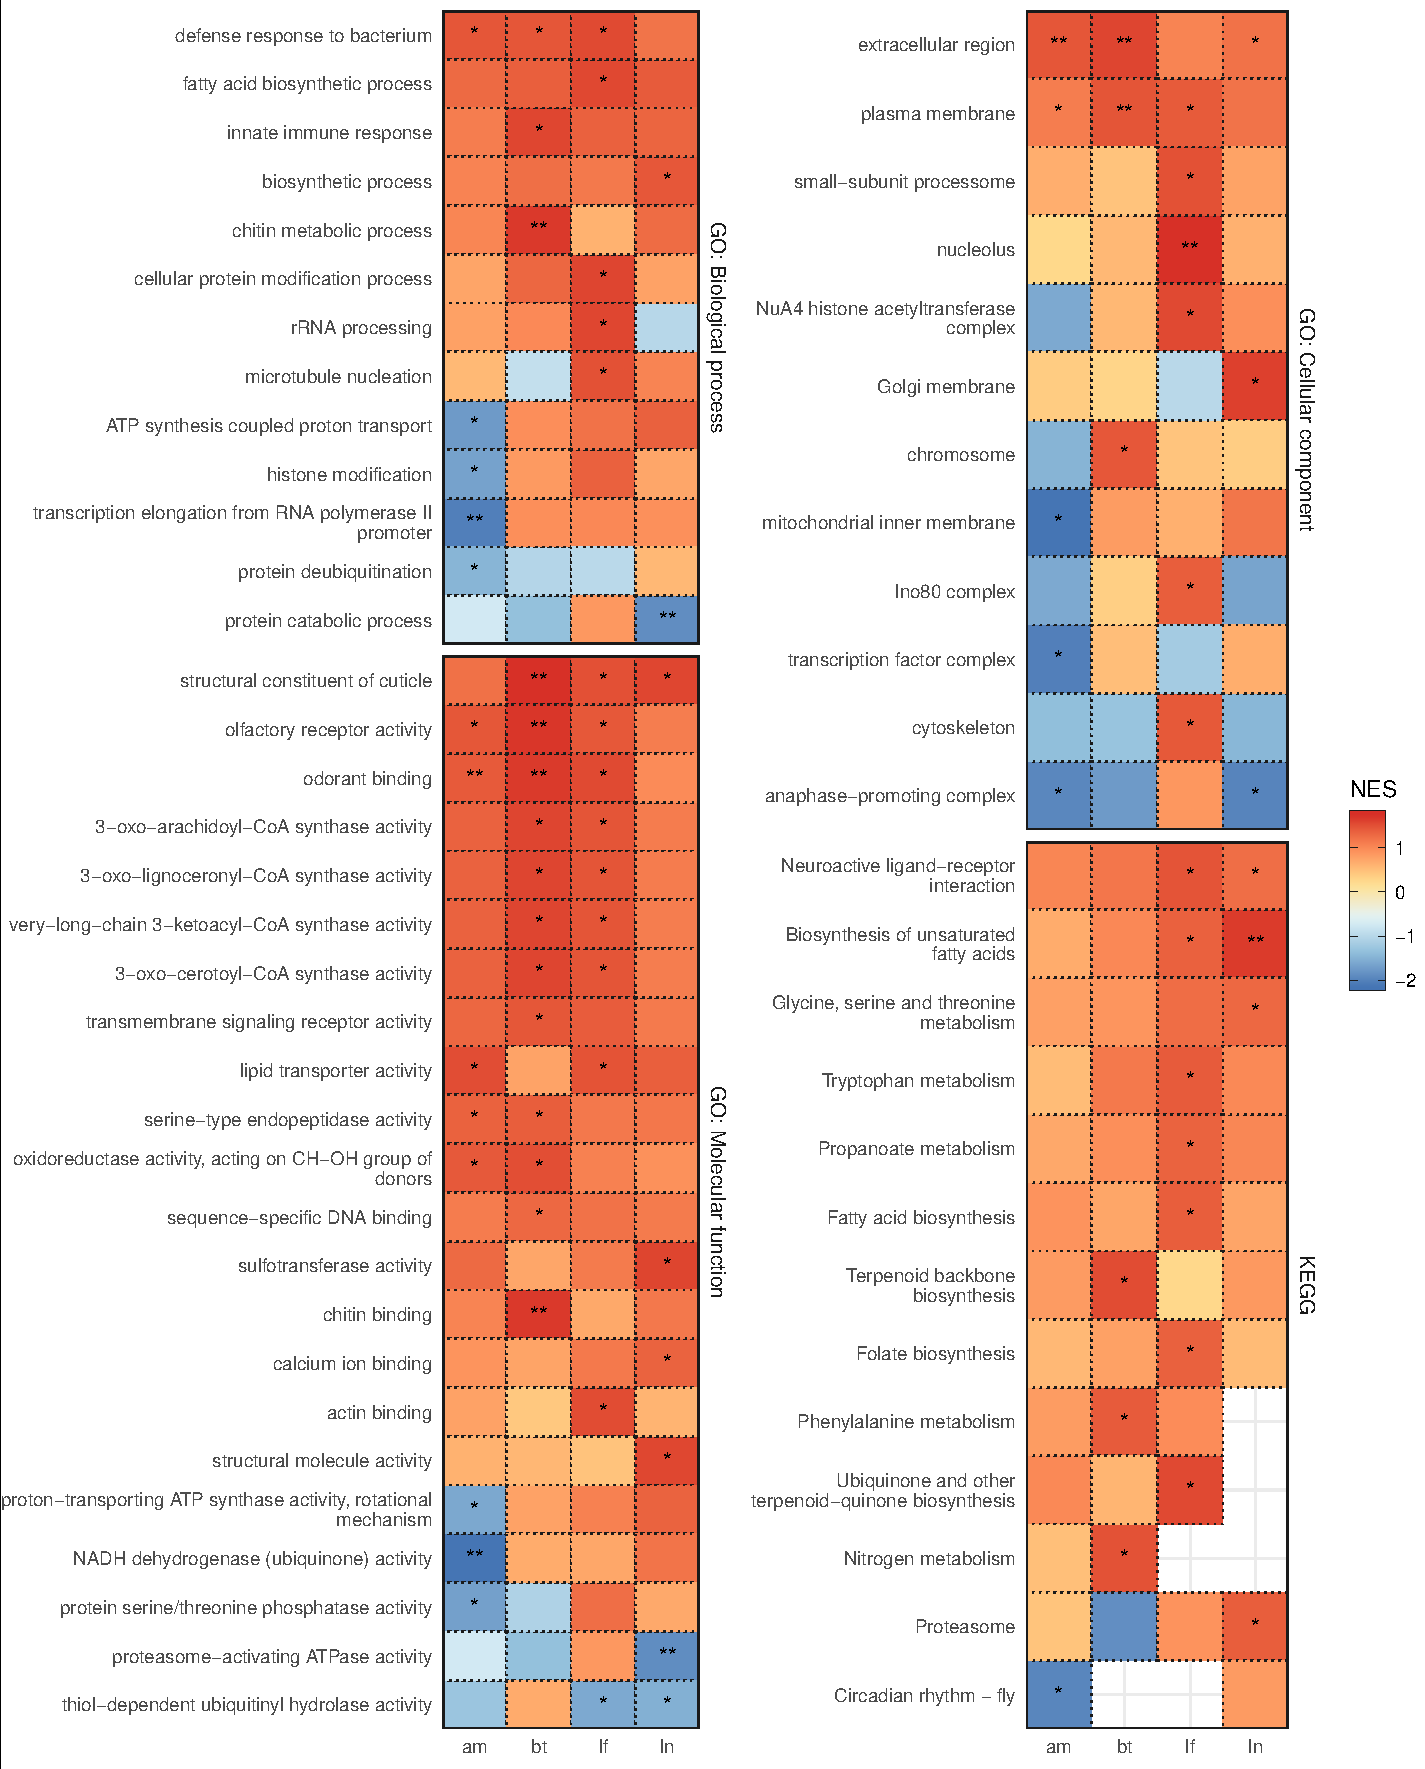
\includegraphics{../figures/MS/Figure 2 - GO and KEGG.pdf}
\caption{\footnotesize Results of Gene Set Enrichment Analysis showing
all Gene Ontology (GO) and Kyoto Encyclopedia of Genes and Genomes
(KEGG) terms that were significantly overrepresented (red) or
underrepresented (blue) among pheromone-sensitive genes in at least one
of the four species. The colour shows the normalised expression score
from gene set enrichment analysis. Asterisks denote statistically
significant enrichment (p \textless{} 0.05), and double asterisks mark
results that remained significant after Benjamini-Hochberg correction.
Empty squares denote cases where we were unable to measure expression
for at least 5 genes annotated with the focal term in one of the
species. \label{fig2}}
\end{figure}

\subsection{Effects of queen pheromone on alternative
splicing}\label{effects-of-queen-pheromone-on-alternative-splicing}

Roughly 20\% of genes had \(\ge2\) detectable isoforms, in all four
species (Figure S4), allowing us to test for pheromone-sensitive
splicing. Pheromone treatment significantly elevated the expression of
one isoform and repressed expression of another isoform for 52 genes in
\emph{A. mellifera}, 55 genes in \emph{L. niger}, 22 genes in \emph{L.
flavus}, and no genes in \emph{B. terrestris} (\autoref{fig1}; Tables
S10-S12). Three genes showed pheromone-sensitive splicing in more than
one species, corresponding to around 4\% of the maximum numbers of genes
that could have overlapped (\autoref{fig1}). Again, these numbers could
well be underestimates, since we have limited power to detect
differential isoform expression, and each `hit' requires two isoforms
per gene to be statistically significant (i.e.~we need 4 significant
results to detect a single overlap between species). \emph{DNA
methyltransferase 3} showed significantly pheromone-sensitive splicing
in \emph{L. niger}, recalling our previous qPCR result that queen
pheromone affects DNA methyltransferase expression\textsuperscript{16}.

We next ranked all the alternatively-spliced genes with detectable
orthologs in all four species in order of the sensitivity of their
isoform profile to pheromone treatment (defined as the range in log fold
change of the focal gene's isoforms), and performed gene set enrichment
analysis on the resulting `splicing sensitivity score'. Most GO and KEGG
terms were enriched in similar patterns across species, e.g.
\emph{intracellular signal transduction}, \emph{transmembrane
transport}, \emph{transcription, DNA-templated}, and \emph{serine-type
endopeptidase activity} (Figure S6; Tables S21-S22). The GO terms
showing non-significant trends toward enrichment included signal
transduction, methyltransferase activity, mRNA processing, protein
transport and modification, and microtubule motor activity. There was
also a positive correlation between species in our measure of the
sensitivity of splicing to pheromone treatment for all six possible
species pairs, though only 2/6 of these correlations were significant
(Table S21). The correlation was esepcially strong for the two bees
(\(\rho\) = 0.19, FDR-corrected p \textless{} \(10^{-7}\)), and was also
signficant for \emph{Bombus} and \emph{Lasius flavus} (\(\rho\) = 0.09,
FDR-corrected p = 0.030). These results suggest that queen pheromone
affects the splicing of some of the same loci across species.

\subsection{Pheromone-sensitive genes tend to pre-date the split between
ants and
bees}\label{pheromone-sensitive-genes-tend-to-pre-date-the-split-between-ants-and-bees}

In all four species, the average pheromone sensitivity (i.e.~absolute
log fold difference between treatments) of ``ancient'' genes (i.e.~those
with a detectable ortholog in both ants and bees) was approximately
double that of genes that are putatutively specific to bees or ants
(Mann-Whitney tests, p \textless{} \(10^{-15}\); Online Supplementary
Material). This result suggests that most pheromone-sensitive genes
existed prior to the evolutionary divergence of bees and ants, and thus
pre-date the origin of eusociality.

\subsection{Effects of queen pheromone on the gene coexpression
network}\label{effects-of-queen-pheromone-on-the-gene-coexpression-network}

Among the 3465 genes for which orthologs were detected in all four
species, we identified nine modules of coexpressed genes, each
containing between 38 and 1639 genes; only 3\% genes were left
unassigned to a module (Figures 1C and 3; Tables S24-S33). The
best-fitting multivariate model of the 9 modules' `eigengenes' (a metric
that quantifies the relative expression of entire modules; see Methods)
contained Treatment as a predictor, but not Species or the Treatment
\(\times\) Species interaction (posterior model probability was
\textgreater{}99\%, indicating clear rejection of the Treatment
\(\times\) Species interaction, and the two models not containing
Treatment; Table S13). This result suggests that some modules of
coexpressed genes responded to pheromone treatment, and that the
response is consistent across species. Specifically, modules 1, 4 and 9
showed a statistically significant difference in mean eigengenes between
pheromone treatments (Figures 1C and 3; Table S14).

\begin{figure}
\centering
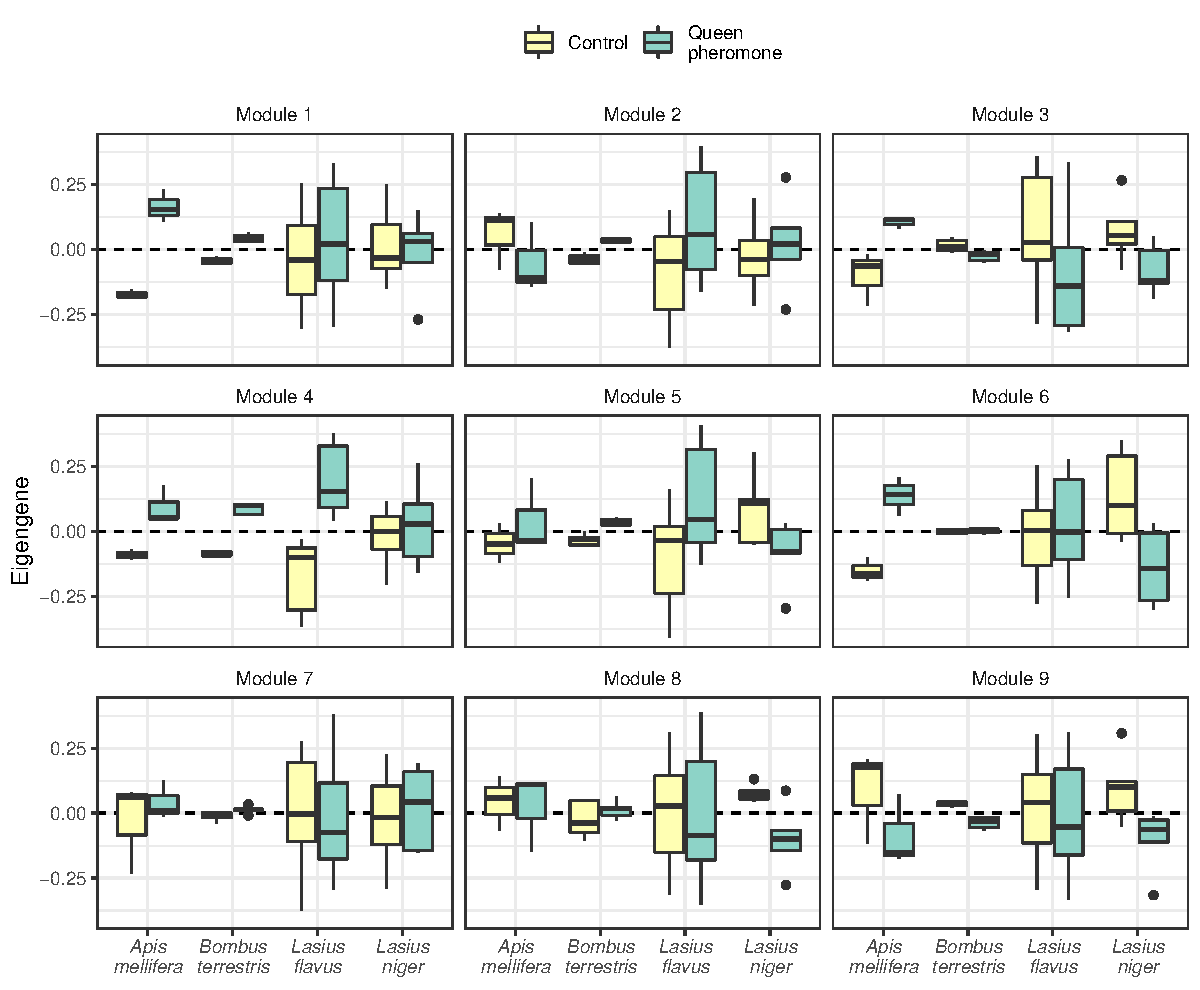
\includegraphics{../figures/MS/Figure 3 - Module eigengenes.pdf}
\caption{\footnotesize Boxplots showing the distribution of `eigengenes'
across samples for each of the nine transcriptional modules identified
via weighted gene coexpression analysis. The eigengene is a measure of
the expression level of a transcriptional module, relative to other
samples in the set. Queen pheromone treatment had a statistically
significant effect across species for modules 1, 4 and 9 (the
annotations give Cohen's d effect size and its 95\% CIs, estimated from
a multivariate Bayesian model of all nine modules). \label{fig3}}
\end{figure}

The pheromone-sensitive module 1 was large (1639 genes), and was
enriched for GO and KEGG terms related to the cell cycle, DNA repair,
transcription and splicing of RNA, and ribosomes (Figures 4 and S7-S9;
Table S23). Module 1 also contained genes relating to the epigenome,
such as \emph{DNA methyltransferase 3} and several histone deacetylases
and methyltransferases. Module 4 (288 genes) was enriched for GO terms
relating to the pentose phosphate pathway, fatty acid and amino acid
biosynthesis, lipid metabolism, vesicle-mediated transport, and for
genes associated with the endoplasmic reticulum (where proteins, lipids,
and steroid horomones are made). This module also contained genes for
synthesising very long-chained fatty acids and acetyl-CoA, which are
precursor substances for the synthesis of cuticular
hydrocarbons\textsuperscript{26,27} and the main components of honeybee
queen mandibular pheromone\textsuperscript{28}. Module 9 was enriched
for purine metabolism; purines are required for cell division and
transcription, and to produce important biomolecules like ATP, NADH, and
coenzyme A.

\begin{figure}
\centering
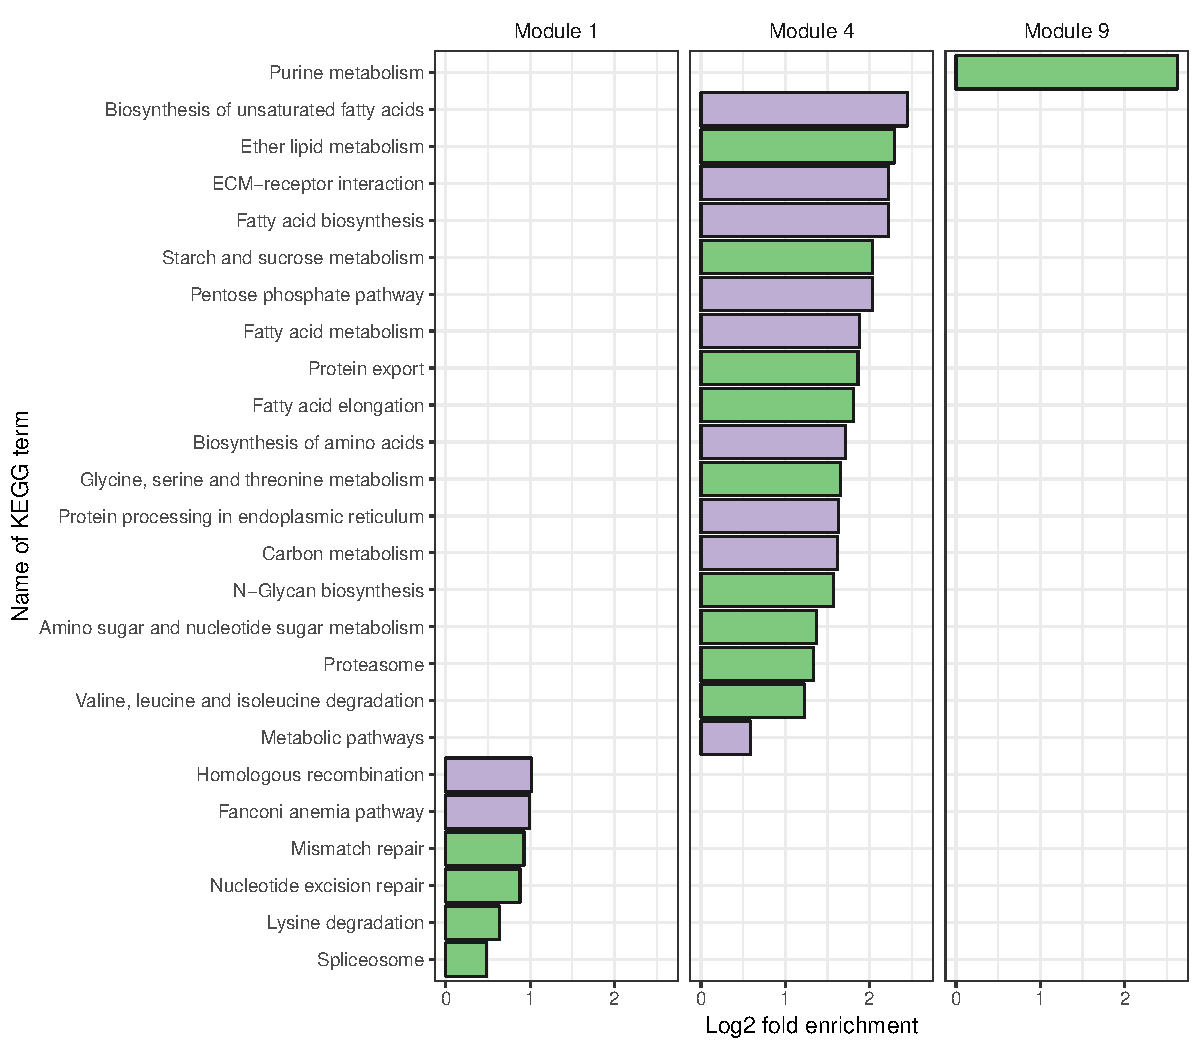
\includegraphics{../figures/MS/Figure 4 - module KEGG.pdf}
\caption{Results of KEGG pathway enrichment analysis for the genes in
each of the three significantly pheromone-sensitive transcriptional
modules. The gene universe was defined as all genes for which we found
an ortholog in all four species (i.e.~the set that was used to discover
these co-expressed modules). All KEGG terms shown in green were
significantly enriched (p \textless{} 0.05), and those shown in purple
remained significant after correction for multiple testing. Fold
enrichment was calculated as the proportion of genes associated with the
focal KEGG term in the module, divided by the equivalent proportion in
the gene universe. Figures S7-S9 show equivalent GO enrichment results.
\label{fig4}}
\end{figure}

\subsection{Pheromone-sensitive genes have low
connectedness}\label{pheromone-sensitive-genes-have-low-connectedness}

We found a negative correlation between sensitivity to queen pheromone
and connectedness across genes (Spearman's \(\rho\) \textgreater{} 0.24,
p \textless{} \(10^{-48}\) for all species). This means that highly
pheromone-sensitive genes are expressed comparatively independently of
the rest of the transcriptome, while highly connected genes tend to be
insensitive to queen pheromone. This result is illustrated by the excess
of pheromone-sensitive genes in Module 0 (which holds the few genes that
were expressed relatively independently of Modules 1-9) in Figure 1C.

\subsection{\texorpdfstring{Characteristics of pheromone-sensitive genes
in \emph{Apis
mellifera}}{Characteristics of pheromone-sensitive genes in Apis mellifera}}\label{characteristics-of-pheromone-sensitive-genes-in-apis-mellifera}

\autoref{fig5} summarises the correlations across genes for a number of
gene-level properties, for honeybees. On average, strongly
pheromone-sensitive genes had less gene body DNA methylation, lower
expression levels, and lower codon usage bias. Pheromone-sensitive genes
had higher values of \(\gamma\), meaning that they have been under
stronger positive selection and/or weaker purifying
selection\textsuperscript{29}. We also found a positive relationship
between pheromone sensitivity and the extent to which a gene was
upregulated in queens relative to sterile workers (as measured
in\textsuperscript{30}). We did not find a significant correlation
between a gene's pheromone sensitivity and the caste-specificity of its
histone modifications (averaged across the gene, using published ChIPseq
data\textsuperscript{31}). However, almost all variables were strongly
inter-correlated (\autoref{fig5}), making the causal relationships among
them (if any) difficult to infer without further evidence.

\begin{figure}
\centering
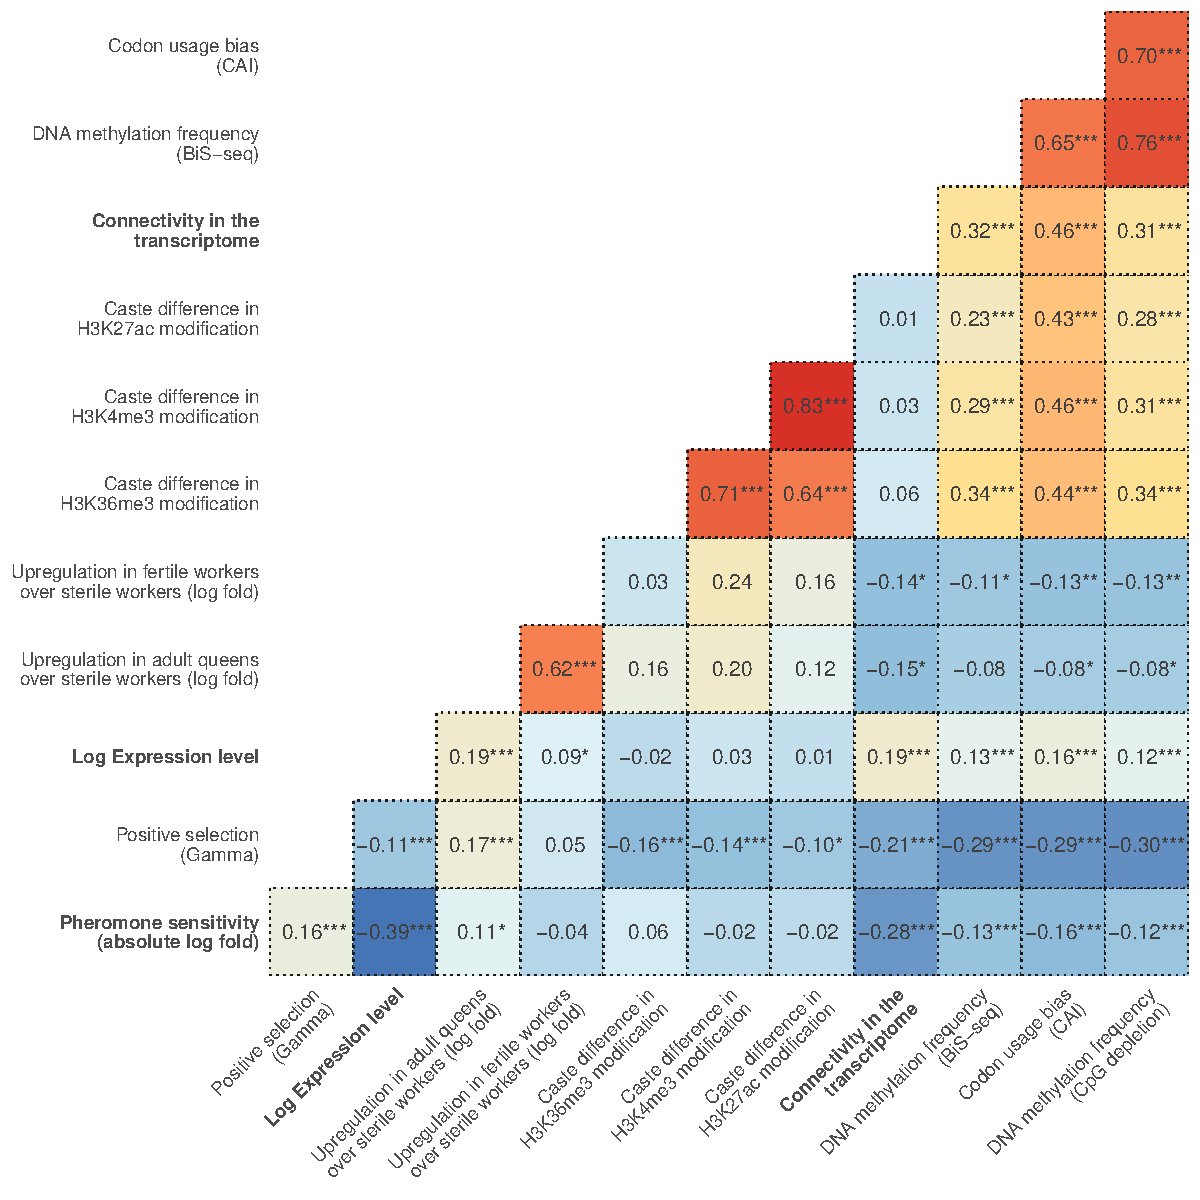
\includegraphics{../figures/MS/Figure 5 - correlations.pdf}
\caption{\footnotesize Spearman correlations for various gene-level
measurements from the present study and earlier research, for \emph{Apis
mellifera} (measurements from the present study are shown in bold).
`Pheromone sensitivity' was calculated as the absolute value of the
Log\(_2\) fold difference in expression between pheromone treatment and
the control. Expression level shows the logarithm of the average across
our 6 \emph{Apis} libraries. For the `Upregulation in queens/fertile
workers' data\textsuperscript{17}, positive values denote genes that
have higher expression in queens or fertile workers, relative to sterile
workers. For the three histone modification
variables\textsuperscript{31}, high values indicate that the
modification is more abundant in queen-destined larvae, and low values
indicate it is more abundant in worker-destined larvae. The two DNA
methylation variables give two different measures of the amount of gene
body DNA methylation, namely an indirect measure (-log CpG O/E ratio)
and a direct measure (BiS-seq\textsuperscript{32}). Codon usage bias was
estimated using the codon adaptation index: high values indicate bias
for particular synonymous codons. Lastly, the parameter gamma
(\(\gamma\)) describes the form of selection, where positive values
denote positive selection, and negative values purifying
selection\textsuperscript{29}. The asterisks indicate the p-values after
FDR correction (* p \textless{} 0.05; ** p \textless{} 0.01; *** p
\textless{} 0.0001). \label{fig5}}
\end{figure}

\subsection{Comparison with caste-specific gene expression in
ants}\label{comparison-with-caste-specific-gene-expression-in-ants}

Hypergeometric tests revealed six instances in which one of our gene
co-expression modules overlapped significantly with one of the modules
from Morandin et al.'s study\textsuperscript{33} of caste-biased gene
expression in ants, after correcting for multiple testing (Table S16).
Modules 2, 3, and 8 from our study overlapped with worker-biased
modules, and Modules 1 and 4 overlapped with queen-biased modules. Since
Modules 1 and 4 are pheromone-sensitive (\autoref{fig3}), these results
suggest that the set of pheromone-sensitive genes overlaps with the set
of caste-biased genes, in ants (as well as bees; \autoref{fig5}). Ten
genes were found in both our Module 4 and Morandin et al.'s queen-biased
module (Table S14); these genes included \emph{protein takeout-like},
\emph{NAD kinase 2, mitochondrial-like}, \emph{histone H2A-like} and
\emph{methyltransferase-like}, again implicating \emph{takeout},
metabolism, and epigenetic processes in caste polyphenism and the
response to queen pheromone.

\section{Discussion}\label{discussion}

To a first approximation, queen pheromones had similar effects on the
transcriptome in all four species. For example, orthologous genes in
bees and ants tended to show similar levels of pheromone sensitivity,
and we identified three transcriptional modules showing a consistent
response to queen pheromone across species. Accordingly, gene set
enrichment analysis revealed that broadly similar functional categories
of genes were enriched in bees and ants. This cross-family conservation
is not unexpected, given that queen pheromones induce similar phenotypes
(e.g.~sterility) in both taxa. However, this outcome was not a foregone
conclusion, for example because bees and ants evolved eusociality
independently (and have few caste-specific genes in
common\textsuperscript{34}), and because bumblebees have smaller, annual
colonies in which behavioral interactions play a larger role in
regulating reproductive division of labour\textsuperscript{35}.

In \emph{Apis} and both \emph{Lasius} species, we found that queen
pheromone treatment caused statistically significant changes in
alternative splicing at multiple loci, increasing the expression of
certain isoforms while inhibiting that of others. The lack of a
significant effect in \emph{B. terrestris} might well be a false
negative, since the estimated sensitivity of alternative splicing to
queen pheromone was strongly correlated across pairs of orthologous
\emph{Apis} and \emph{Bombus} genes. Also, \emph{Bombus} genes with high
(though non-significant) pheromone-sensitive splicing were significantly
enriched for similar GO and KEGG terms as those in the other three
species (Figure S6). Our study thus adds to the growing list of cases in
which alternative splicing underlies polyphenisms in
insects\textsuperscript{22,36--38}.

In \emph{Apis}, pheromone-sensitive genes tended to be positively
selected, weakly connected in the transcriptional network, weakly
expressed, and hypomethylated, relative to pheromone-insensitive genes.
Additionally, queen pheromones affected a somewhat similar set of genes
to that which distinguishes adult queens and workers in bees as well as
ants, consistent with our prediction that queen pheromones would make
gene expression more worker-like. Finally, pheromone-sensitive genes
were disproportionately likely to pre-date the divergence of bees and
ants, consistent with their patterns of enrichment for GO and KEGG terms
associated with taxonomically ubiquitous processes such as lipid
biosynthesis.

Many genes or gene families were differentially expressed in two or more
species. As one example, queen pheromone inhibited the expression of
major royal jelly proteins (MRJPs) in honeybees (echoing earlier
findings that MRJPs expression covaries with reproductive
physiology\textsuperscript{39}) and in \emph{L. niger}. Among other
functions, MRJPs are essential for rearing new queens, which workers do
when their current queen dies or becomes infertile (i.e.~when the queen
pheromone disappears)\textsuperscript{8}. MRJPs are produced during
development and in the adult fat body, and belong to the
phylogenetically ancient \emph{yellow} gene family\textsuperscript{40},
which has diverse roles in development, the nervous system, behaviour,
immunity, and pigmentation.

Genes related to synthesis and transport of lipids and fatty acids
formed a strongly co-expressed transcriptional module, which was
modulated by queen pheromone across taxa. The affected genes included
enzymes for making long-chained fatty acids and fatty acyl-CoAs, which
are biosynthetic precursors of cuticular hydrocarbons (CHCs) as well as
the components of the queen mandibular pheromone (QMP) of
honeybees\textsuperscript{26--28}. Additionally, a number of genes
putatively involved in CHC and QMP biosynthesis, such as cytochrome
P450s, NADPH synthases, and genes involved in fatty acid elongation and
oxidoreductase activity\textsuperscript{26--28,41}, were differentially
expressed. We also observed large (though non-significant) effects of
queen pheromone on the expression of \emph{vitellogenin} (a lipid
transporter) and \emph{hexamerin 70a precursor}, two classic
`eusociality genes' that have been linked to caste and oogenesis by many
previous studies (e.g.\textsuperscript{42,43}). These results are
expected given that pheromone-deprived workers begin depositing yolk in
their ovaries via lipid synthesis and transport\textsuperscript{44}.

Our results hint at the mechanism by which queen pheromones achieve
their effects, and suggest a novel (and heretofor
missing\textsuperscript{12,14}) mechanism underlying the widely-observed
honest signalling of fecundity via olfactory cues/signals in social
insects. This honest signalling is considered a puzzle because of the
apparent fitness benefits of exaggerating one's fecundity via pheromones
(in queens) or of `covert' reproduction without pheromonal signalling
(in workers)\textsuperscript{1,5,12,14,45}. We speculate that the fatty
acid-derived queen pheromones found in ants and bees are absorbed
directly into the body (e.g.~by ingestion), where they inhibit lipid
biosynthesis via negative feedback, thereby inhibiting oogenesis. If
this hypothesis proves correct, the colony could be regarded as having a
shared `social physiology', whereby colony members keep track of their
own physiological state via standard within-body signals (e.g.~juvenile
hormone, insulin signalling), as well of the states of other individuals
via pheromones\textsuperscript{46}. We also speculate that workers
evolved elevated sensitivity to queen pheromones as colony sizes
increased over evolutionary time, e.g.~via changes in olfaction and
physiology, allowing them to continue to express the sterility response
even though their contact with the queen is reduced. Lastly, the
necessity of lipid synthesis and transport for oogenesis, coupled with
an inextricable, non-evolvable link between the makeup of the internal
and external lipid profiles, would enforce a reliable correlation
between individual fecundity and odour profile\textsuperscript{5,12}.

In another notable result, the gene \emph{protein takeout-like} was
among the most strongly pheromone-sensitive genes in all four species.
The \emph{takeout} family encodes proteins that are expressed in, and
secreted from, the brain-associated fat body and antennae, and some
members putatively bind juvenile hormone\textsuperscript{47}.
Interestingly, \emph{takeout} genes have been linked to discrete
polyphenisms in termites\textsuperscript{48},
locusts\textsuperscript{49} and aphids\textsuperscript{50}, suggesting
that they might be similarly important to polymorphism in the eusocial
Hymenoptera. Additionally, in \emph{Drosophila}, the expression of
\emph{takeout} is stimulated by the male-typical isoforms of the sex
differentiation genes \emph{doublesex} and \emph{fruitless}, and
suppressed by the female isoforms\textsuperscript{51}. This is
noteworthy in light of the recently-proposed hypothesis that sex
differentiation genes such as \emph{doublesex} have been co-opted to
control caste polyphenism in eusocial insects\textsuperscript{20--22}.
This finding also brings to mind the `reproductive groundplan
hypothesis'\textsuperscript{46}, which posits that reproductive division
of labour is the result of regulatory evolution of nutrition signalling
pathways, e.g.~insulin-like signalling, which (among other things)
controls the balances of lipid and sugar synthesis and metabolism, and
the rate of ageing (which differs between queens and workers, and
between fertile and sterile workers\textsuperscript{24}).

Additionally, \emph{serotonin receptor} was among the most
pheromone-sensitive genes in all four species. Serotonin seems
understudied in social insects, although two studies have found
differences in serotonin titre or receptor gene expression between
sterile and fertile workers, in \emph{Polistes}
wasps\textsuperscript{52} and \emph{Apis}\textsuperscript{53}. Another
biogenic amine --- dopamine --- is better-studied; it has been
implicated in the response to queen pheromone in
\emph{Apis}\textsuperscript{54}, and affects behaviour and fecundity in
many insects\textsuperscript{55--57}. There was also some evidence that
the expression of the neurohormone corazonin was modulated by queen
pheromone (e.g.~Table S17), consistent with experimental results showing
that corazonin induces worker-like behaviors and suppresses queen-like
behaviors in an ant\textsuperscript{58}.

Several genes related to myosin, which functions in muscle contraction,
were significantly downregulated in the queen pheromone treatment in at
least one species. Interestingly, a recent study compared the
transcriptomes of queens and workers in 16 ant species with RNA-seq, and
found only a single gene that was significantly differentially expressed
between castes in all 16 species: another myosin
gene\textsuperscript{33}. Myosin genes are also differentially expressed
between fertile and sterile workers\textsuperscript{59,60} and queen-
and worker- destined larvae\textsuperscript{61} in honeybees, and
between queens and workers in bumblebees\textsuperscript{23}. We
speculate that myosins show caste-specific expression due to caste
differences in muscle morphology and activity levels (e.g.~queen ants
fly while workers do not, and in bees, there is a caste difference in
flight frequency).

The consistently pheromone-sensitive module 1 contained many genes
relating to histone modification, particularly histone-lysine
N-methyltransferases and histone deacetylases. These included
\emph{histone-lysine N-methyltransferase eggless}, which trimethylates
Lys-9 of histone H3 in the \emph{Drosophila} ovary, and which is
essential for oogenesis (FlyBase: FBgn0086908). Another interesting gene
was \emph{male-specific lethal 1 homolog}, which regulates gene
expression by acetlyation of H4 lysine 16; the resulting H4K16ac
`epimark' is hypothesised to regulate the development and renewal of
female germline stem cells\textsuperscript{62}. Another histone
acetlyation epimark, H3K27ac, is related to the major-minor worker size
polymorphism in carpenter ants\textsuperscript{63}, and differs between
queens and workers in honeybees\textsuperscript{31}. In sum, it seems
likely that the receipt of queen pheromone causes a rewiring of the
epigenome, which in turn regulates the genes underlying oogenesis. We
also found that queen pheromone affected the splicing of \emph{DNA
methyltransferase 3} (\emph{dnmt3}) in \emph{Lasius niger}, echoing our
previous work showing that queen pheromones affect the expression of
\emph{dnmt1} and \emph{dnmt3} in bees and ants\textsuperscript{16}, and
again paralleling evidence that differential DNA methylation is involved
in queen-worker polyphenism\textsuperscript{64}. Direct measurement of
the effect of queen pheromone on the epigenome has not yet been
performed (but see\textsuperscript{16}).

A number of recent papers on the origins of eusociality have asked
whether the key genetic players tend to be `ancient' genes with
fundamental cellular functions, or more recently-evolved genes with
specialised functions (e.g.\textsuperscript{33,34,65}). Most of this
work has focused on genes showing queen- or worker-biased expression,
but since that gene set overlaps substantially with the set of
pheromone-sensitive genes, our results are apposite. We found that
pheromone-sensitive genes tend to predate the split between bees and
ants, suggesting that present-day queen pheromones primarily affect
genes that already existed in the genomes of the first eusocial insects.
However, we also found that pheromone-sensitive genes had low
connectedness, expression levels, and codon usage bias; none of these
characteristics are consistent with the targets of queen pheromone being
`housekeeping' genes, i.e.~extremely ancient, constitutively-expressed
genes with ubiquitous cellular functions\textsuperscript{33}. Instead,
queen pheromone affected a moderately-sized subset of the transcriptome,
whose expression varied relatively independently of the remainder. This
result is interesting because genetic modules showing flexible
expression patterns and reduced pleiotropy are predicted to be major
drivers of adaptation because they are comparatively free to undergo
adaptation\textsuperscript{66}. Our results are consistent with a model
whereby a relatively self-contained genetic module (controlling nutrient
homeostasis, and thus oogenesis) acquired a new expression pattern,
producing the observed polyphenism of fertile and sterile females.
Subsequently, the genes in this module underwent adaptation to their new
roles, explaining our result that pheromone-sensitive genes are both
evolutionarily ancient and positively selected.

\section{Methods}\label{methods}

\subsection{RNA sequencing of pheromone-treated bees and
ants}\label{rna-sequencing-of-pheromone-treated-bees-and-ants}

The present study uses RNA obtained from the same insect samples as
those used in an earlier study\textsuperscript{16}, which provides
complete methods for the pheromone bioassay, RNA extraction, and
preparation of cDNA. Briefly, we treated nest boxes containing workers
from 3-8 colonies per species with either a solvent-only control or
their own species' queen pheromone, and then extracted total RNA from
individual workers (either whole bodies, or a random lateral body half
for \emph{Bombus}), removed genomic DNA with DNase, and
reverse-transcribed RNA to cDNA. For \emph{Apis mellifera} honeybees,
the pheromone used was commercially available Queen Mandibular Pheromone
(QMP), which is a mixture of 5 chemicals (principally keto acids). For
\emph{Bombus terrestris}, the pheromone was the CHC pentacosane
(C\(_{25}\)), and for the two \emph{Lasius} ant species it was the CHC
3-methylhentriacontane (3-MeC\(_{31}\)). The \emph{B. terrestris}
workers were from the same cohort and colonies as in
Holman\textsuperscript{67}, though they were different individuals.

We then used Qubit fluorometry to determine the mass of cDNA obtained
from each worker, and pooled equal amounts of cDNA from five
randomly-selected workers for each combination of species, colony, and
treatment. Not including 4 problematic samples that were later discarded
(see Figures S1-S2), we sequenced 44 cDNA pools (6 for \emph{A.
mellifera}, 10 for \emph{B. terrestris}, 13 for \emph{L. flavus}, and 10
for \emph{L. niger}; Table S1); library preparation (using Illumina
TruSeq kits) and sequencing was conducted by Edinburgh Genomics. The
libraries were sequenced in three lanes of an Illumina HiSeq 2500
sequencer set to high output, yielding 125bp paired-end reads. All
samples were individually barcoded and run in all three lanes,
preventing lane effects from confounding the experiment. The experiment
yielded 14±1.3 (st. dev.), 12.3±4.3, 14.7±2.7, 13.1±1.4 million reads
for \emph{A. mellifera}, \emph{B. terrestris}, \emph{L. flavus} and
\emph{L. niger}, respectively. We used Trimmomatic\textsuperscript{68}
to remove sequencing primers, and trimmed reads for quality using the
SLIDINGWINDOW:4:15 parameter prior to subsequent analyses. After
trimming, the number of paired reads was 10.8±1, 8.3±2.9, 10.2±1.4,
10.8±1.3 million, respectively.

\subsection{Quantifying differences in gene expression or alternative
splicing between pheromone
treatments}\label{quantifying-differences-in-gene-expression-or-alternative-splicing-between-pheromone-treatments}

We aligned and quantified the raw reads using the
RSEM\textsuperscript{69} pipeline with Bowtie2\textsuperscript{70} to
transcripts from published genomes for \emph{A. mellifera}, \emph{B.
terrestris} and \emph{L. niger}\textsuperscript{71--73}. The \emph{L.
niger} genome assembly had no isoform information, so we identified
isoforms using Tophat\textsuperscript{74}. No reference genome was
available for \emph{L. flavus}, so we assembled the transcriptome
\emph{de novo} using Trinity\textsuperscript{75}, and identified coding
regions with TransDecoder\textsuperscript{76}.

Within each species, we used EBSeq-HMM\textsuperscript{77} to calculate
the fold difference in expression between the control and
pheromone-treated workers for each transcript using the rsem-run-ebseq
pipeline implemented in Trinity. We adjusted p-values to control the
false discovery rate using the Benjamini-Hochberg method, then defined
genes with adjusted p\textless{}0.05 as significantly differentially
expressed. As a sensitivity analysis, we re-ran the EBSeq analysis after
removing low-abundance transcripts, increasing power by reducing the
number of tests; we obtained essentially identical lists of significant
genes to those from the full analysis.

To identify genes whose splicing was significantly affected by queen
pheromone, we searched for genes for which at least one isoform was
significantly upregulated in the control, while another isoform was
significantly downregulated. We also calculated a `pheromone sensitivity
of splicing' score, by taking the maximum difference in log fold change
for the isoforms of each gene (e.g.~a gene with three isoforms showing
-2, +0.1, and +1 log fold difference between treatments would score 3).
This score was use to test for correlations across species in the
gene-level sensitivity of splicing to pheromone, and for GO and KEGG
enrichment tests of pheromone-sensitive splicing (see below).

\subsection{Testing for conserved effects of queen pheromone across
species}\label{testing-for-conserved-effects-of-queen-pheromone-across-species}

The simplest method to identify conserved effects on gene expression is
to tally the number of orthologous genes showing significant
differential expression in two or more species (as in the Venn diagrams
in Figure 1). Though robust, this method is highly conservative, because
one has finite statistical power to detect any given differentially
expressed gene. Power issues are compounded when searching for genes
that show a conserved response across species, since one needs to avoid
two or more false negatives per locus. We therefore performed two
additional formal analyses to test for conserved transcriptional effects
of queen pheromones, as well as plotting the pheromone sensitivity for
each gene (Figure 1C) to allow qualitative assessment of the extent of
cross-species similarity.

For the first formal test, we tested whether the pheromone sensitivity
of each gene is correlated in each pair of species, using Spearman's
rank correlation on pairs of orthologous genes (see Figures 1C; 1D).
Pheromone sensitivity was defined as the absolute log fold difference in
expression between treatments. This test has improved power relative to
the Venn diagram appraoch, but does not reveal the number or identity of
the conserved/convergent pheromone-sensitive genes.

Secondly, we identified the genes that had detectable orthologs in all
four species (defining orthologs as genes that were each other's best
BLAST hit, with both e-values \(<10^{-4}\)), and then ranked them from
most to least pheromone-sensitive within each species. Then, we asked
which genes appeared in the top \(n\)-most pheromone sensitive genes in
all four species, for \(n\)=100, 200\ldots{} 500. This analysis has good
power to identify candidate genes that responded to pheromones in all
four species, but runs the risk of false positives (i.e.~genes that
topped all four gene lists by chance alone).

\subsection{Evolutionary age of pheromone-sensitive
genes}\label{evolutionary-age-of-pheromone-sensitive-genes}

To test whether pheromone-sensitive genes tend to have an ancient or
recent evolutionarily origin, we classified genes as either `ancient' or
`putatively family-specific' using reciprocal best BLAST. Bee genes
(\emph{Apis} or \emph{Bombus}) with a BLAST hit (e-value \(10^{-4}\)) in
at least one of the ant species were classified as ancient, and
\emph{vice versa}. Genes that were not classified as ancient might be
false negatives (e.g.~due to gaps in our sequence data, or because genes
were lost in one lineage), hence our caution in labelling genes as
family-specific. Any misclassifications should make it harder to detect
a difference between pheromone-sensitive and -insensitive genes, but
could not produce a spurious difference.

\subsection{Gene co-expression network
analysis}\label{gene-co-expression-network-analysis}

We constructed a gene co-expression network for all four species, which
included all genes for which orthologs were detected in all species,
following Morandin et al.\textsuperscript{33}. The aim of this analysis
was to search for `modules' of co-expressed genes that change their
expression in response to queen pheromone in all the species. We
therefore used an empirical Bayes method\textsuperscript{78}
(implemented via the ComBat function in R's \emph{sva}
package\textsuperscript{79}) to transform the expression data so as to
remove multivariate differences in expression attributable to species or
colony, clarifying the effect of pheromone treatment on the
transcriptome.

We used the R package WGCNA\textsuperscript{80} to define the gene
co-expression network and identify transcriptional modules, largely
using the default settings. The two exceptions were that we imposed a
minimum size for transcriptional modules of 30 genes, and used a signed
(rather than unsigned) coexpression network. These choices mean that our
analysis recovers modules of 30+ genes that are all simultaneously up-
or down-regulated across our 44 samples.

To test whether species, treatment, and their interaction explained
variation in module `eigengenes' (a metric describing the expression
level of a particular module in the focal sample, relative to the other
samples\textsuperscript{80}), we used Bayesian multivariate models
implemented in the R package \texttt{brms}\textsuperscript{81}. We fit
five candidate models, all with the 9 eigengenes as a multivariate
response, colony as a random effect, and Gaussian errors. The five
models differed in their fixed effects, and we compared the models' fits
in order to test for significant effects of treatment, species, and
their interaction (using posterior model probabilities, calculated using
bridge sampling).

We also used the co-expression network to calculate connectedness for
all genes. We defined connectedness as the sum of the correlations in
expression between a given gene and every other gene in the
network\textsuperscript{82}. Thus, a `highly-connected gene' is one
whose expression varies in concert with many other genes, across
samples.

\subsection{GO and KEGG enrichment
analyses}\label{go-and-kegg-enrichment-analyses}

We downloaded Kyoto Encyclopedia of Genes and Genomes (KEGG) from the
KEGG API and gene ontology (GO) terms from NCBI, for the best-annotated
of our four species, \emph{Apis mellifera}. KEGG terms group together
genes that are known to interact in biochemical pathways, while GO
classifies genes by Biological Process, Molecular Function, or Cellular
Component. Genes in non-\emph{Apis} species were assumed to have the
same GO and KEGG terms as their reciprocal best BLAST hits in \emph{A.
mellifera}.

We implemented Kolmogorov-Smirnov enrichment tests (also called Gene Set
Enrichment Analysis or GSEA\textsuperscript{83}) using the
\texttt{fgsea} package for R. These tests rank all genes in the set
under test (called the `gene universe') in order of some metric of
interest, and then identify GO or KEGG terms that are significantly
over- and under-represented among the top-ranked genes, relative to
bootstrapped random expectations. As well as presenting the uncorrected
p-values, we corrected the GO and KEGG results for multiple testing
using the Benjamini-Hochberg method, though we note that this approach
is crude and probably overly-conservative, since tests of the different
terms are not independent. GO results were simplified by collapsing
redundant GO terms into higher-order ones using the
\texttt{collapsePathways} function in \texttt{fgsea}.

To identify enriched GO and KEGG terms among genes whose expression was
sensitive to pheromone treatment, we ranked genes by the log\_\{10\}
posterior probability of differential expression (computed by EBSeq-HMM)
and defined the gene universe as all genes (for \emph{Apis}) or all
genes with a detectable ortholog in \emph{Apis} (for other species). To
identify enriched terms among genes with pheromone-sensitive splicing,
we ranked genes by their splicing score, and specified the gene universe
as all alternatively-spliced genes with \emph{Apis} orthologs.

To identify enriched GO and KEGG terms for each of the 9 co-expressed
genetic modules, we used standard hypergeometric tests (implemented in
the \texttt{clusterProfiler} R package), and defined the gene universe
as all 3465 genes used in the coexpression network analysis.

\subsection{\texorpdfstring{Characteristics of pheromone-sensitive genes
in
\emph{Apis}}{Characteristics of pheromone-sensitive genes in Apis}}\label{characteristics-of-pheromone-sensitive-genes-in-apis}

\emph{Apis mellifera} honeybees are well-studied relative to our other
species, and so we compared our pheromone sensitivity and connectedness
data to pre-existing gene-level data from \emph{A. mellifera} using
Spearman correlations.

First, we used published microarray results\textsuperscript{30} to test
whether pheromone-sensitive genes also showed a large difference in
expression between A) queens and sterile workers, and B) fertile workers
and sterile workers. Second, we examined codon usage bias, as measured
by the codon adaptation index\textsuperscript{84}; high values indicate
a bias towards particular synonymous codons in the coding regions of a
gene. Third, we tested for relationships with the frequency of DNA
methylation within the gene body, using two complementary measures of
DNA methylation: the amount of CpG depletion (measured as the negative
log observed/expected CpG ratio), or the percentage of methylated
cytosines, estimated using whole genome bisulphite
sequencing\textsuperscript{32}. Fourth, we tested whether
pheromone-sensitive genes show signatures of positive or purifying
selection since the split between \emph{A. mellifera} and its congeneric
\emph{A. cerana}, using the metric \(\gamma\)\textsuperscript{29}.
Lastly, we tested whether pheromone-sensitivity was correlated with the
log expression level of each gene, using the average expression levels
from the present study.

\subsection{Comparison with caste-specific gene expression in
ants}\label{comparison-with-caste-specific-gene-expression-in-ants-1}

Using reciprocal best BLAST (e-value \(10^{-4}\)), we attempted to
classify the groups of orthologous genes from our study into one of the
orthologous gene groups defined for queens and workers from 16 ant
species in Morandin et al.\textsuperscript{33}. We then tested for
significant overlap between that study's 36 gene co-expression modules,
and the modules from our own study, using hypergeometric tests on all
possible pairs of modules (followed by FDR correction). We thereby
tested whether the groups of coexpressed genes that respond to pheromone
also tend to show differential expression between queens and workers.

\subsection{Data availability and
reproducibility}\label{data-availability-and-reproducibility}

The sequencing data have been deposited at NCBI (BioSample ascensions:
SAMD00106316-58). Bash, Python, and R scripts used to reproduce our
bioinformatics pipeline and data analysis are archived at Github
(\url{https://github.com/mikheyev/queen-pheromone}). As well as the
supplementary figures and tables, our Online Supplementary Material
contains the R scripts used to generate each result (the supplement can
also be viewed online:
\url{https://mikheyev.github.io/queen-pheromone}).

\section{Acknowledgements}\label{acknowledgements}

We are very grateful to Lijun Qiu, Tapio Envall, Sini Vuorensyrjä, Heini
Ali-Kovero and Minna Tuominen for laboratory assistance, to Soojin Yi
and Brendan Hunt for sharing data, and to Mark and Kirsten Holman for
beekeeping. Brian Hanley and Jocelyn Millar kindly provided synthetic
3-MeC\(_{31}\). Claire Morandin and Tim Linksvayer provided helpful
discussion.

\section{Funding}\label{funding}

This work received funding from the Research School of Biology at
Australian National University to LH; a Discovery Project (DP170100772)
to LH and ASM; the Kone Foundation to HH; the Academy of Finland to HH
(135970, 127390), and the Center of Excellence in Biological
Interactions (284666).

\section{References}\label{references}

\hypertarget{refs}{}
\hypertarget{ref-VanOystaeyen:2014vr}{}
1. Van Oystaeyen, A. \emph{et al.} Conserved class of queen pheromones
stops social insect workers from reproducing. \emph{Science}
\textbf{343,} 287--290 (2014).

\hypertarget{ref-Holman:2018tx}{}
2. Holman, L. Queen pheromones and reproductive division of labour: a
meta-analysis. \emph{Behavioural Ecology} \textbf{in press,
doi:10.1093/beheco/ary023,} (2018).

\hypertarget{ref-Slessor:1988cj}{}
3. Slessor, K. N., Kaminski, L.-A., King, G. G. S., Borden, J. H. \&
Winston, M. L. Semiochemical basis of the retinue response to queen
honey bees. \emph{Nature} \textbf{332,} 354--356 (1988).

\hypertarget{ref-Smith:2016dz}{}
4. Smith, A. A., Millar, J. G. \& Suarez, A. V. Comparative analysis of
fertility signals and sex-specific cuticular chemical profiles of
\emph{Odontomachus} trap-jaw ants. \emph{J Exp Biol} \textbf{219,}
419--430 (2016).

\hypertarget{ref-Smith:2009ic}{}
5. Smith, A. A., Hölldobler, B. \& Liebig, J. Cuticular hydrocarbons
reliably identify cheaters and allow enforcement of altruism in a social
insect. \emph{Current Biology} \textbf{19,} 78--81 (2009).

\hypertarget{ref-Yagound:2015ip}{}
6. Yagound, B. \emph{et al.} Fertility signaling and partitioning of
reproduction in the ant \emph{Neoponera apicalis}. \emph{Journal of
Chemical Ecology} \textbf{41,} 557--566 (2015).

\hypertarget{ref-Vargo:1988fv}{}
7. Vargo, E. A bioassay for a primer pheromone of queen fire ants
(\emph{Solenopsis invicta}) which inhibits the production of sexuals.
\emph{Insectes Sociaux} \textbf{35,} 382--392 (1988).

\hypertarget{ref-Winston:1990vi}{}
8. Winston, M. L., Higo, H. A. \& Slessor, K. N. Effect of various
dosages of queen mandibular gland pheromone on the inhibition of queen
rearing in the honey bee (Hymenoptera: Apidae). \emph{Annals of the
Entomological Society of America} \textbf{83,} 234--238 (1990).

\hypertarget{ref-Pankiw:1998vta}{}
9. Pankiw, T., Huang, Z. Y., Winston, M. L. \& Robinson, G. E. Queen
mandibular gland pheromone influences worker honey bee (\emph{Apis
mellifera} L.) foraging ontogeny and juvenile hormone titers.
\emph{Journal of Insect Physiology} \textbf{44,} 685--692 (1998).

\hypertarget{ref-Vergoz:2007ej}{}
10. Vergoz, V., Schreurs, H. A. \& Mercer, A. R. Queen pheromone blocks
aversive learning in young worker bees. \emph{Science} \textbf{317,}
384--386 (2007).

\hypertarget{ref-Keller:1993vl}{}
11. Keller, L. \& Nonacs, P. The role of queen pheromones in social
insects: queen control or queen signal? \emph{Animal Behaviour}
\textbf{45,} 787--794 (1993).

\hypertarget{ref-Holman:2012ey}{}
12. Holman, L. Costs and constraints conspire to produce honest
signalling: Insights from an ant queen pheromone. \emph{Evolution}
2094--2105 (2012).

\hypertarget{ref-Peso:2015hx}{}
13. Peso, M., Elgar, M. A. \& Barron, A. B. Pheromonal control:
reconciling physiological mechanism with signalling theory.
\emph{Biological reviews of the Cambridge Philosophical Society}
\textbf{90,} 542--559 (2015).

\hypertarget{ref-Oi:2015go}{}
14. Oi, C. A. \emph{et al.} The origin and evolution of social insect
queen pheromones: Novel hypotheses and outstanding problems.
\emph{Bioessays} \textbf{37,} 808--821 (2015).

\hypertarget{ref-Peters:2017bk}{}
15. Peters, R. S. \emph{et al.} Evolutionary history of the Hymenoptera.
\emph{Current Biology} \textbf{27,} 1013--1018 (2017).

\hypertarget{ref-Holman:2016ea}{}
16. Holman, L., Trontti, K. \& Helantera, H. Queen pheromones modulate
DNA methyltransferase activity in bee and ant workers. \emph{Biology
Letters} \textbf{12,} 20151038 (2016).

\hypertarget{ref-Grozinger:2003er}{}
17. Grozinger, C. M., Sharabash, N. M., Whitfield, C. W. \& Robinson, G.
E. Pheromone-mediated gene expression in the honey bee brain.
\emph{Proceedings of the National Academy of Sciences of the United
States of America} \textbf{100,} 14519--14525 (2003).

\hypertarget{ref-Fussnecker:2011cg}{}
18. Fussnecker, B. L., McKenzie, A. M. \& Grozinger, C. M. cGMP
modulates responses to queen mandibular pheromone in worker honey bees.
\emph{Journal of Comparative Physiology A} \textbf{197,} 939--948
(2011).

\hypertarget{ref-Foret2012jf}{}
19. Foret, S. \emph{et al.} DNA methylation dynamics, metabolic fluxes,
gene splicing, and alternative phenotypes in honey bees.
\emph{Proceedings of the National Academy of Sciences USA} \textbf{109,}
4968--4973 (2012).

\hypertarget{ref-Klein:2016da}{}
20. Klein, A. \emph{et al.} Evolution of social insect polyphenism
facilitated by the sex differentiation cascade. \emph{PLoS Genetics}
\textbf{12,} e1005952 (2016).

\hypertarget{ref-Johnson:2016ko}{}
21. Johnson, B. R. \& Jasper, W. C. Complex patterns of differential
expression in candidate master regulatory genes for social behavior in
honey bees. \emph{Behavioral Ecology and Sociobiology} \textbf{70,}
1033--1043 (2016).

\hypertarget{ref-velasque2018doublesex}{}
22. Velasque, M., Qiu, L. \& Mikheyev, A. S. The \emph{doublesex} sex
determination pathway regulates reproductive division of labor in honey
bees. \emph{bioRxiv} 314492 (2018).

\hypertarget{ref-Harrison:2015kf}{}
23. Harrison, M. C., Hammond, R. L. \& Mallon, E. B. Reproductive
workers show queenlike gene expression in an intermediately eusocial
insect, the buff-tailed bumble bee \emph{Bombus terrestris}.
\emph{Molecular ecology} \textbf{24,} 3043--3063 (2015).

\hypertarget{ref-Dixon:2014it}{}
24. Dixon, L., Kuster, R. \& Rueppell, O. Reproduction, social behavior,
and aging trajectories in honeybee workers. \emph{Age} \textbf{36,}
89--101 (2014).

\hypertarget{ref-holman2014co}{}
25. Holman, L. Conditional helping and evolutionary transitions to
eusociality and cooperative breeding. \emph{Behavioral Ecology}
\textbf{25,} 1173--1182 (2014).

\hypertarget{ref-Blomquist:2010ux}{}
26. Blomquist, G. J. Biosynthesis of cuticular hydrocarbons. in
\emph{Insect hydrocarbons: Biology, biochemistry and chemical ecology}
(eds. Blomquist, G. J. \& Bagnères, A.-G.) (Cambridge University Press,
2010).

\hypertarget{ref-Dembeck:2015jb}{}
27. Dembeck, L. M. \emph{et al.} Genetic architecture of natural
variation in cuticular hydrocarbon composition in \emph{Drosophila
melanogaster}. \emph{eLife} \textbf{4,} e09861 (2015).

\hypertarget{ref-Wu:2017br}{}
28. Wu, Y. \emph{et al.} Comparative transcriptome analysis on the
synthesis pathway of honey bee (\emph{Apis mellifera}) mandibular gland
secretions. \emph{Scientific Reports} \textbf{7,} (2017).

\hypertarget{ref-Harpur:2014hk}{}
29. Harpur, B. A. \emph{et al.} Population genomics of the honey bee
reveals strong signatures of positive selection on worker traits.
\emph{Proceedings of the National Academy of Sciences of the United
States of America} \textbf{111,} 2614--2619 (2014).

\hypertarget{ref-Grozinger:2007ki}{}
30. Grozinger, C. M., Fan, Y., Hoover, S. E. R. \& Winston, M. L.
Genome-wide analysis reveals differences in brain gene expression
patterns associated with caste and reproductive status in honey bees
(\emph{Apis mellifera}). \emph{Molecular Ecology} \textbf{16,}
4837--4848 (2007).

\hypertarget{ref-wojciechowski2018ph}{}
31. Wojciechowski, M. \emph{et al.} Phenotypically distinct female
castes in honey bees are defined by alternative chromatin states during
larval development. \emph{Genome Research} (2018).

\hypertarget{ref-Galbraith:2016gz}{}
32. Galbraith, D. A. \emph{et al.} Testing the kinship theory of
intragenomic conflict in honey bees (\emph{Apis mellifera}).
\emph{Proceedings of the National Academy of Sciences USA} \textbf{113,}
1020--1025 (2016).

\hypertarget{ref-Morandin:2016jd}{}
33. Morandin, C. \emph{et al.} Comparative transcriptomics reveals the
conserved building blocks involved in parallel evolution of diverse
phenotypic traits in ants. \emph{Genome biology} \textbf{17,} 43 (2016).

\hypertarget{ref-Berens:2015hg}{}
34. Berens, A. J., Hunt, J. H. \& Toth, A. L. Comparative
transcriptomics of convergent evolution: different genes but conserved
pathways underlie caste phenotypes across lineages of eusocial insects.
\emph{Molecular Biology and Evolution} \textbf{32,} 690--703 (2015).

\hypertarget{ref-doorn1989fa}{}
35. Van Doorn, A. Factors influencing dominance behaviour in queenless
bumblebee workers (\emph{Bombus terrestris}). \emph{Physiological
Entomology} \textbf{14,} 211--221 (1989).

\hypertarget{ref-kijimoto2012div}{}
36. Kijimoto, T., Moczek, A. P. \& Andrews, J. Diversification of
\emph{doublesex} function underlies morph-, sex-, and species-specific
development of beetle horns. \emph{Proceedings of the National Academy
of Sciences} \textbf{109,} 20526--20531 (2012).

\hypertarget{ref-wang2014lo}{}
37. Wang, X. \emph{et al.} The locust genome provides insight into swarm
formation and long-distance flight. \emph{Nature Communications}
\textbf{5,} 2957 (2014).

\hypertarget{ref-zhuo2017tra}{}
38. Zhuo, J.-C. \emph{et al.} \emph{Tra-2} mediates crosstalk between
sex determination and wing polyphenism in female \emph{Nilaparvata
lugens}. \emph{Genetics} \textbf{207,} 1067--1078 (2017).

\hypertarget{ref-thompson2008ge}{}
39. Thompson, G. J., Kucharski, R., Maleszka, R. \& Oldroyd, B. P.
Genome-wide analysis of genes related to ovary activation in worker
honey bees. \emph{Insect Molecular Biology} \textbf{17,} 657--665
(2008).

\hypertarget{ref-Drapeau:2006jt}{}
40. Drapeau, M. D., Albert, S., Kucharski, R., Prusko, C. \& Maleszka,
R. Evolution of the Yellow/Major Royal Jelly Protein family and the
emergence of social behavior in honey bees. \emph{Genome Research}
\textbf{16,} 1385--1394 (2006).

\hypertarget{ref-hasegawa2009di}{}
41. Hasegawa, M. \emph{et al.} Differential gene expression in the
mandibular glands of queen and worker honeybees, \emph{Apis mellifera
L.}: implications for caste-selective aldehyde and fatty acid
metabolism. \emph{Insect Biochemistry and Molecular Biology}
\textbf{39,} 661--667 (2009).

\hypertarget{ref-Nelson:2007fz}{}
42. Nelson, C. M., Ihle, K. E., Fondrk, M. K., Page, R. E. \& Amdam, G.
V. The gene \emph{vitellogenin} has multiple coordinating effects on
social organization. \emph{PLoS Biology} \textbf{5,} 673--677 (2007).

\hypertarget{ref-Martins:2011co}{}
43. Martins, J. R., Anhezini, L., Dallacqua, R. P., Zilá L. P. Simões \&
Bitondi, M. M. G. A honey bee hexamerin, HEX 70a, is likely to play an
intranuclear role in developing and mature ovarioles and testioles.
\emph{PLoS ONE} \textbf{6,} e29006 (2011).

\hypertarget{ref-CruzLandim:2006uz}{}
44. Cruz-Landim, C., Patrício, K. \& Antonialli, W. F. Cell death and
ovarian development in highly eusocial bees (Hymenoptera, Apidae): Caste
differentiation and worker egg laying. \emph{Braz J Morphol Sci}
\textbf{23,} 27--42 (2006).

\hypertarget{ref-Holman:2013iy}{}
45. Holman, L., Linksvayer, T. A. \& d'Ettorre, P. Genetic constraints
on dishonesty and caste dimorphism in an ant. \emph{American Naturalist}
\textbf{181,} 161--170 (2013).

\hypertarget{ref-johnson2010de}{}
46. Johnson, B. R. \& Linksvayer, T. A. Deconstructing the
superorganism: Social physiology, groundplans, and sociogenomics.
\emph{Quarterly Review of Biology} \textbf{85,} 57--79 (2010).

\hypertarget{ref-Hagai:cp}{}
47. Hagai, T., Cohen, M. \& Bloch, G. Genes encoding putative
Takeout/juvenile hormone binding proteins in the honeybee (\emph{Apis
mellifera}) and modulation by age and juvenile hormone of the
takeout-like gene GB19811. \emph{Insect Biochemistry and Molecular
Biology} \textbf{37,} 689--701

\hypertarget{ref-Hojo:2005ht}{}
48. Hojo, M., Morioka, M., Matsumoto, T. \& Miura, T. Identification of
soldier caste-specific protein in the frontal gland of nasute termite
\emph{Nasutitermes takasagoensis} (Isoptera: Termitidae). \emph{Insect
Biochemistry and Molecular Biology} \textbf{35,} 347--354 (2005).

\hypertarget{ref-Guo:2011ks}{}
49. Guo, W. \emph{et al.} \emph{CSP} and \emph{takeout} genes modulate
the switch between attraction and repulsion during behavioral phase
change in the migratory locust. \emph{PLoS Genetics} \textbf{7,}
e1001291 (2011).

\hypertarget{ref-Ghanim:2006bb}{}
50. Ghanim, M., Dombrovsky, A., Raccah, B. \& Sherman, A. A microarray
approach identifies \emph{ANT}, \emph{OS-D} and \emph{takeout-like}
genes as differentially regulated in alate and apterous morphs of the
green peach aphid \emph{Myzus persicae} (Sulzer). \emph{Insect
Biochemistry and Molecular Biology} \textbf{36,} 857--868 (2006).

\hypertarget{ref-Dauwalder:2002ga}{}
51. Dauwalder, B., Tsujimoto, S., Moss, J. \& Mattox, W. The
\emph{Drosophila} \emph{takeout} gene is regulated by the somatic
sex-determination pathway and affects male courtship behavior.
\emph{Genes \& Development} \textbf{16,} 2879--2892 (2002).

\hypertarget{ref-sasaki2007ne}{}
52. Sasaki, K., Yamasaki, K. \& Nagao, T. Neuro-endocrine correlates of
ovarian development and egg-laying behaviors in the primitively eusocial
wasp (\emph{Polistes chinensis}). \emph{Journal of Insect Physiology}
\textbf{53,} 940--949 (2007).

\hypertarget{ref-vergoz2012bio}{}
53. Vergoz, V., Lim, J. \& Oldroyd, B. Biogenic amine receptor gene
expression in the ovarian tissue of the honey bee \emph{Apis mellifera}.
\emph{Insect Molecular Biology} \textbf{21,} 21--29 (2012).

\hypertarget{ref-Beggs:2007dm}{}
54. Beggs, K. T. \emph{et al.} Queen pheromone modulates brain dopamine
function in worker honey bees. \emph{Proceedings of the National Academy
of Sciences of the United States of America} \textbf{104,} 2460--2464
(2007).

\hypertarget{ref-McQuillan:2012ir}{}
55. McQuillan, H. J., Barron, A. B. \& Mercer, A. R. Age- and
behaviour-related changes in the expression of biogenic amine receptor
genes in the antennae of honey bees (\emph{Apis mellifera}).
\emph{Journal of Comparative Physiology A: Sensory Neural and Behavioral
Physiology} \textbf{198,} 753--761 (2012).

\hypertarget{ref-Okada:2015cg}{}
56. Okada, Y. \emph{et al.} Social dominance and reproductive
differentiation mediated by dopaminergic signaling in a queenless ant.
\emph{J Exp Biol} \textbf{218,} 1091--1098 (2015).

\hypertarget{ref-Weitekamp:2017if}{}
57. Weitekamp, C. A., Libbrecht, R. \& Keller, L. Genetics and evolution
of social behavior in insects. \emph{Annual Review of Genetics}
\textbf{51,} 219--239 (2017).

\hypertarget{ref-gospocic2017ne}{}
58. Gospocic, J. \emph{et al.} The neuropeptide corazonin controls
social behavior and caste identity in ants. \emph{Cell} \textbf{170,}
748--759 (2017).

\hypertarget{ref-Cardoen:2011dn}{}
59. Cardoen, D. \emph{et al.} Genome-wide analysis of alternative
reproductive phenotypes in honeybee workers. \emph{Molecular ecology}
\textbf{20,} 4070--4084 (2011).

\hypertarget{ref-Niu:2014gu}{}
60. Niu, D. \emph{et al.} Transcriptome comparison between inactivated
and activated ovaries of the honey bee \emph{Apis mellifera} L.
\emph{Insect Molecular Biology} \textbf{23,} 668--681 (2014).

\hypertarget{ref-Barchuk:2007vs}{}
61. Barchuk, A., Cristino, A. \& Kucharski, R. Molecular determinants of
caste differentiation in the highly eusocial honeybee \emph{Apis
mellifera}. \emph{BMC Developmental Biology} \textbf{7,} 70 (2007).

\hypertarget{ref-sun2015his}{}
62. Sun, J. \emph{et al.} Histone h1-mediated epigenetic regulation
controls germline stem cell self-renewal by modulating h4k16
acetylation. \emph{Nature Communications} \textbf{6,} 8856 (2015).

\hypertarget{ref-simola2016epi}{}
63. Simola, D. F. \emph{et al.} Epigenetic (re) programming of
caste-specific behavior in the ant \emph{Camponotus floridanus}.
\emph{Science} \textbf{351,} aac6633 (2016).

\hypertarget{ref-Kucharski:2008gu}{}
64. Kucharski, R., Maleszka, J., Foret, S. \& Maleszka, R. Nutritional
control of reproductive status in honeybees via DNA methylation.
\emph{Science} \textbf{319,} 1827--1830 (2008).

\hypertarget{ref-Patalano:2015vl}{}
65. Patalano, S. \emph{et al.} Molecular signatures of plastic
phenotypes in two eusocial insect species with simple societies.
\emph{Proceedings of the National Academy of Sciences} \textbf{112,}
13970--13975 (2015).

\hypertarget{ref-Gerhart:2007eq}{}
66. Gerhart, J. \& Kirschner, M. The theory of facilitated variation.
\emph{Proceedings of the National Academy of Sciences USA} \textbf{104,}
8582--8589 (2007).

\hypertarget{ref-Holman:2014jq}{}
67. Holman, L. Bumblebee size polymorphism and worker response to queen
pheromone. \emph{PeerJ} \textbf{2,} e604 (2014).

\hypertarget{ref-Bolger:2014ek}{}
68. Bolger, A. M., Lohse, M. \& Usadel, B. Trimmomatic: a flexible
trimmer for Illumina sequence data. \emph{Bioinformatics} \textbf{30,}
2114--2120 (2014).

\hypertarget{ref-Li:2011cb}{}
69. Li, B. \& Dewey, C. N. RSEM: accurate transcript quantification from
RNA-Seq data with or without a reference genome. \emph{BMC
Bioinformatics} \textbf{12,} 323 (2011).

\hypertarget{ref-Langmead:2012ka}{}
70. Langmead, B. \& Salzberg, S. L. Fast gapped-read alignment with
Bowtie 2. \emph{Nature Methods} \textbf{9,} 357--359 (2012).

\hypertarget{ref-Consortium:2006wj}{}
71. The Honeybee Genome Sequencing Consortium. Insights into social
insects from the genome of the honeybee \emph{Apis mellifera}.
\emph{Nature} \textbf{443,} 931--949 (2006).

\hypertarget{ref-BenMSadd:2015bq}{}
72. Sadd, B. M. \emph{et al.} The genomes of two key bumblebee species
with primitive eusocial organization. \emph{Genome Biology} \textbf{16,}
76 (2015).

\hypertarget{ref-Konorov:2017ft}{}
73. Konorov, E. A. \emph{et al.} Genomic exaptation enables \emph{Lasius
niger} adaptation to urban environments. \emph{BMC Evolutionary Biology}
\textbf{17,} 39 (2017).

\hypertarget{ref-Trapnell:2009dp}{}
74. Trapnell, C., Pachter, L. \& Salzberg, S. L. TopHat: discovering
splice junctions with RNA-Seq. \emph{Bioinformatics} \textbf{25,}
1105--1111 (2009).

\hypertarget{ref-Grabherr:2011jb}{}
75. Grabherr, M. G. \emph{et al.} Full-length transcriptome assembly
from RNA-Seq data without a reference genome. \emph{Nature
Biotechnology} \textbf{29,} 644--652 (2011).

\hypertarget{ref-Haas:2013jq}{}
76. Haas, B. J. \emph{et al.} De novo transcript sequence reconstruction
from RNA-seq using the Trinity platform for reference generation and
analysis. \emph{Nature Protocols} \textbf{8,} 1494--1512 (2013).

\hypertarget{ref-Leng:2015dw}{}
77. Leng, N. \emph{et al.} EBSeq-HMM: a Bayesian approach for
identifying gene-expression changes in ordered RNA-seq experiments.
\emph{Bioinformatics} \textbf{31,} 2614--2622 (2015).

\hypertarget{ref-johnson:2007adj}{}
78. Johnson, W. E., Li, C. \& Rabinovic, A. Adjusting batch effects in
microarray expression data using empirical bayes methods.
\emph{Biostatistics} \textbf{8,} 118--127 (2007).

\hypertarget{ref-Leek:2012ee}{}
79. Leek, J. T., Johnson, W. E., Parker, H. S., Jaffe, A. E. \& Storey,
J. D. The sva package for removing batch effects and other unwanted
variation in high-throughput experiments. \emph{Bioinformatics}
\textbf{28,} 882--883 (2012).

\hypertarget{ref-Langfelder:2008bd}{}
80. Langfelder, P. \& Horvath, S. WGCNA: an R package for weighted
correlation network analysis. \emph{BMC Bioinformatics} \textbf{9,} 559
(2008).

\hypertarget{ref-burkner2017brms}{}
81. Bürkner, P.-C. \& others. brms: An R package for Bayesian multilevel
models using Stan. \emph{Journal of Statistical Software} \textbf{80,}
1--28 (2017).

\hypertarget{ref-Masalia:2017ki}{}
82. Masalia, R. R., Bewick, A. J. \& Burke, J. M. Connectivity in gene
coexpression networks negatively correlates with rates of molecular
evolution in flowering plants. \emph{PLoS ONE} \textbf{12,} e0182289
(2017).

\hypertarget{ref-subramanian2005gene}{}
83. Subramanian, A. \emph{et al.} Gene set enrichment analysis: A
knowledge-based approach for interpreting genome-wide expression
profiles. \emph{Proceedings of the National Academy of Sciences}
\textbf{102,} 15545--15550 (2005).

\hypertarget{ref-Sharp:1987tz}{}
84. Sharp, P. M. \& Li, W. H. The codon adaptation index - a measure of
directional synonymous codon usage bias, and its potential applications.
\emph{Nucleic Acids Research} \textbf{15,} 1281--1295 (1987).


\end{document}
